% !TEX root = main.tex

\subsection{仿真模拟}
\qquad 设置时钟周期为100ns,初始30ns为准备时间,然后将Reset设为1使其开始工作。仿真结果见图\ref{fig:wave_1}到图\ref{fig:wave_15},每条指令的说明均已附在波形图之下。可以看见仿真结果与预期结果相同。
\begin{enumerate}
    \item \verb'0x00  addiu $1,$0,8'\\
    IF(0)状态的后半周期读入指令,并写入指令寄存器IR;WB(7)状态的后半周期将结果8写入Reg[1]
    \item \verb'0x04  ori $2,$0,2'\\
    WB(7)状态后半周期将结果2写入Reg[2]
\begin{figure}[H]
\centering
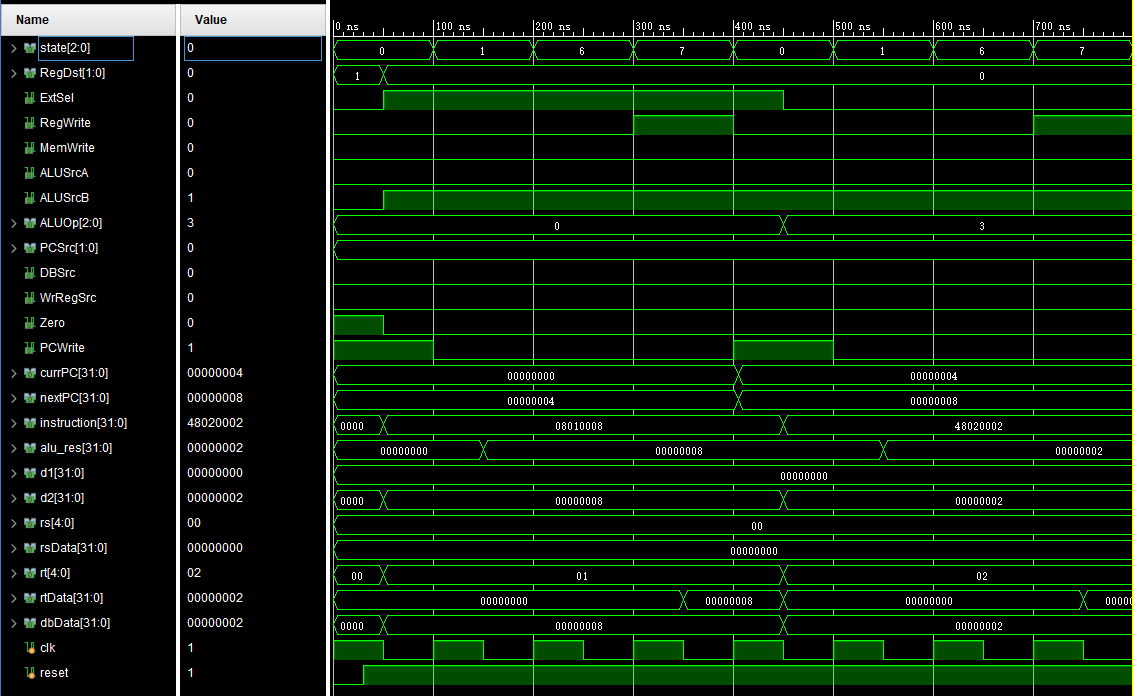
\includegraphics[width=0.9\linewidth]{fig/FullIns/Ins1.PNG}
\caption{波形图1}
\label{fig:wave_1}
\end{figure}
    \item \verb'0x08  xori $3,$2,8'\\
    ID(1)状态读入Reg[2]=2,与立即数8异或,即$1000 \mathrm{xor} 0010 = 1010 = (10)_{10}$;WB(7)状态将结果$(A)_{16}$写入Reg[3]
    \item \verb'0x0C  sub $4,$3,$1'\\
    WB(7)状态将结果$\mathrm{Reg}[3]-\mathrm{Reg}[1]=10-8=2$写入Reg[4]
\begin{figure}[H]
\centering
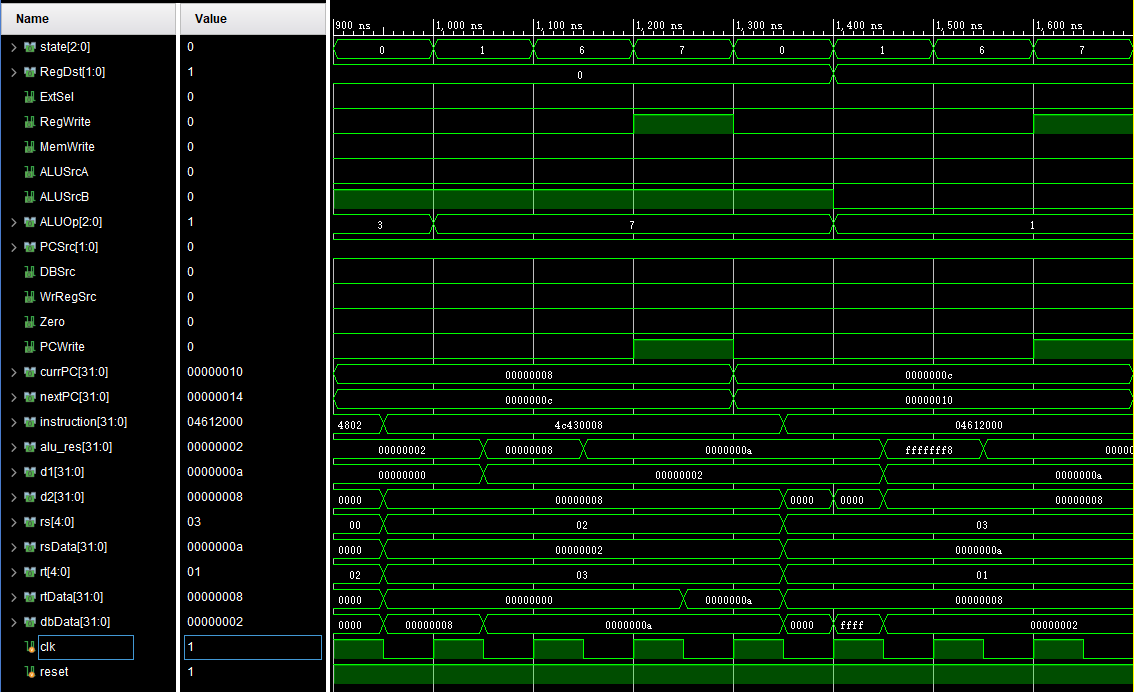
\includegraphics[width=0.9\linewidth]{fig/FullIns/Ins2.PNG}
\caption{波形图2}
\label{fig:wave_2}
\end{figure}
    \item \verb'0x10  and $5,$4,$2'\\
    WB(7)状态将结果$\mathrm{Reg}[4]\&\mathrm{Reg}[2]=2\&2=2$写入Reg[5]
    \item \verb'0x14  sll $5,$5,2'\\
    WB(7)状态将结果$\mathrm{Reg}[5]<<2=2<<2=8$写入Reg[5]
\begin{figure}[H]
\centering
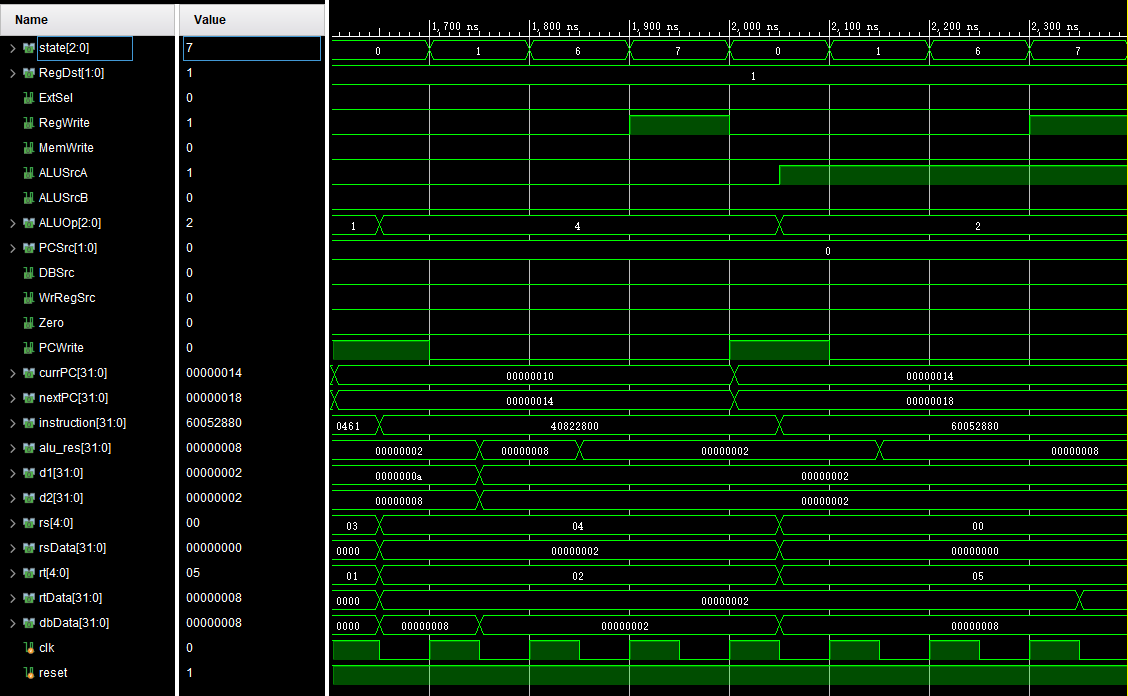
\includegraphics[width=0.9\linewidth]{fig/FullIns/Ins3.PNG}
\caption{波形图3}
\label{fig:wave_3}
\end{figure}
    \item \verb'0x18  beq $5,$1,-2'\\
    EXE(5)状态ALU结果为$\mathrm{Reg}[5]-\mathrm{Reg}[1]=8-8=0==0$,跳转回\verb'0x14'
    \item \verb'0x14  sll $5,$5,2'\\
    WB(7)状态将结果$\mathrm{Reg}[5]<<2=8<<2=32=(20)_{16}$写入Reg[5]
\begin{figure}[H]
\centering
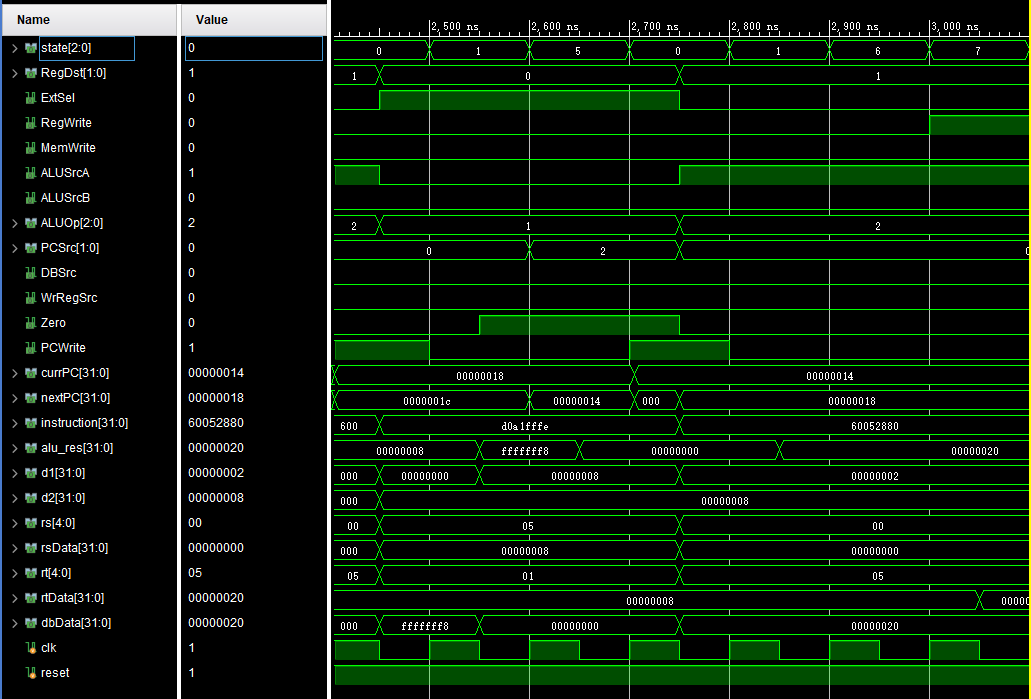
\includegraphics[width=0.9\linewidth]{fig/FullIns/Ins4.PNG}
\caption{波形图4}
\label{fig:wave_4}
\end{figure}
    \item \verb'0x18  beq $5,$1,-2'\\
    EXE(5)状态ALU结果为$\mathrm{Reg}[5]-\mathrm{Reg}[1]=32-8=24=(18)_{16}\ne 0$,不跳转,执行下一指令
    \item \verb'0x1C  jal 0x0000050'\\
    调用子程序,IF(0)状态更新下一PC值为\verb'0x50';ID(1)状态RegDst为2,对Reg[31]写入原来的PC+4,即\verb'0x20',故图中ALU在ID(1)状态的后半周期值回改变,因为RegFile写入了新的值
\begin{figure}[H]
\centering
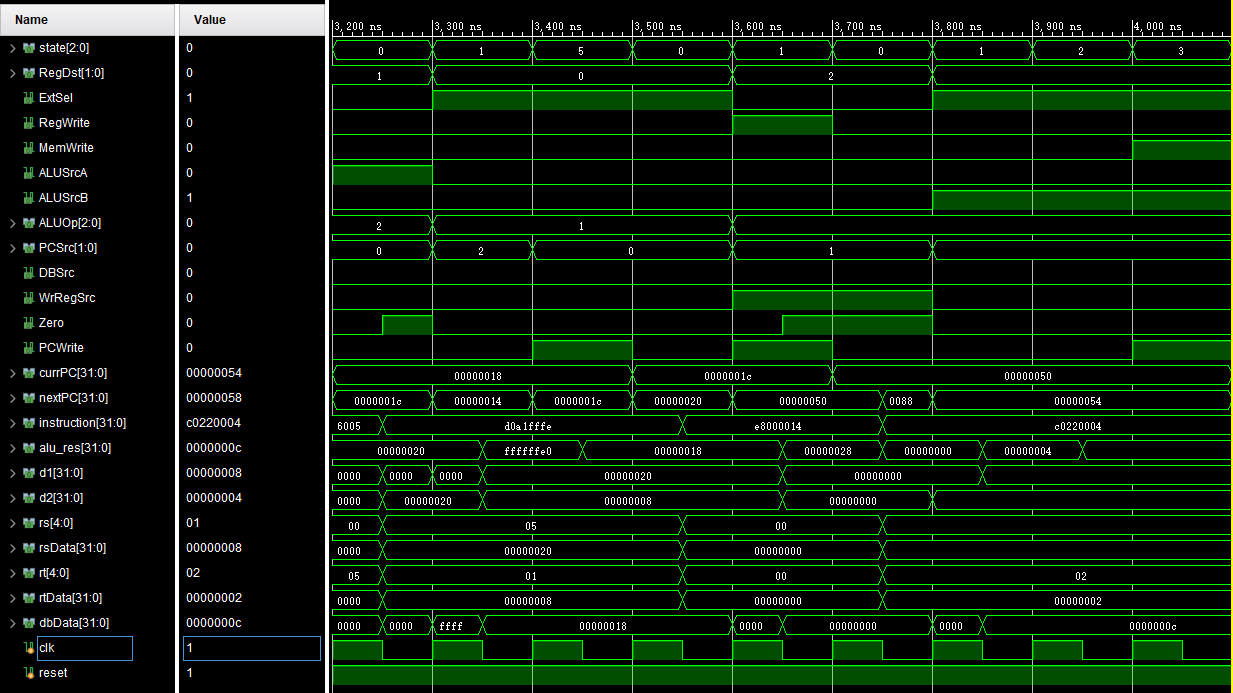
\includegraphics[width=0.8\linewidth]{fig/FullIns/Ins5.PNG}
\caption{波形图5}
\label{fig:wave_5}
\end{figure}
    \item \verb'0x50  sw $2,4($1)'\\
    将Reg[2]=2存入$\text{Mem}[\text{Reg}[1]+4]=\text{Reg}[12]=\text{Mem}[(C)_{16}]$
    \item \verb'0x54  lw $13,4($1)'\\
    将$\text{Mem}[12]=2$取出,在WB(4)状态存入Reg[13]
\begin{figure}[H]
\centering
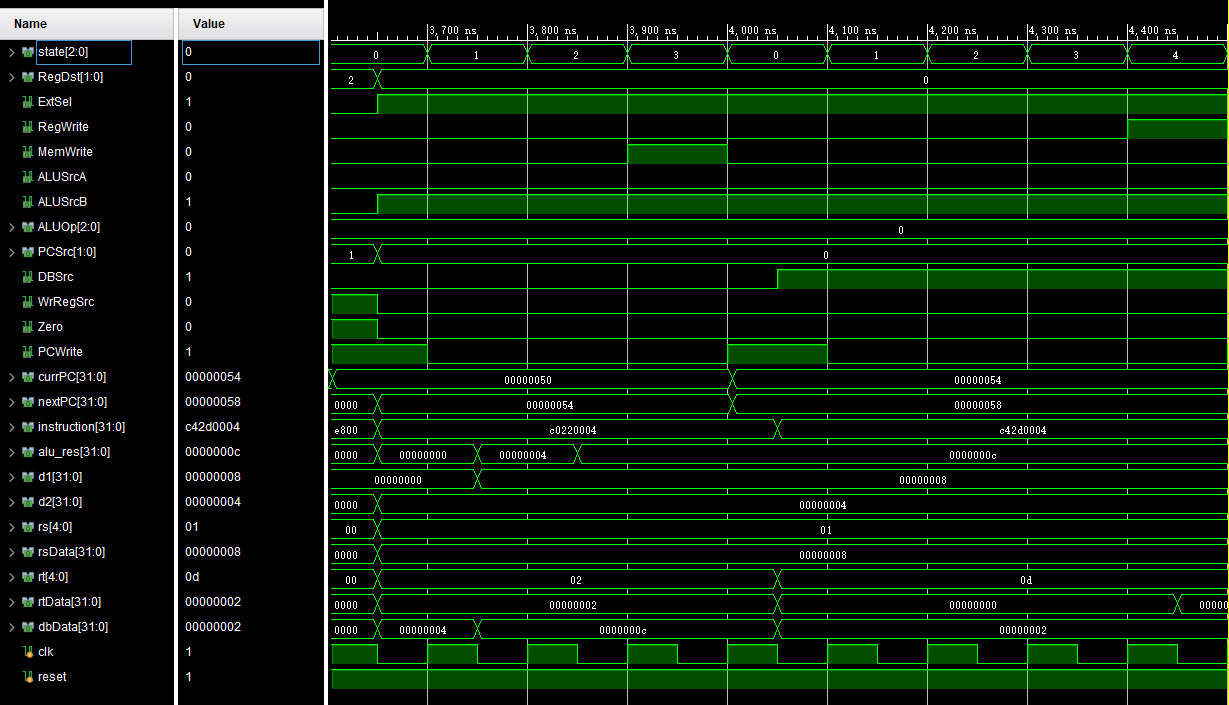
\includegraphics[width=0.9\linewidth]{fig/FullIns/Ins6.PNG}
\caption{波形图6}
\label{fig:wave_6}
\end{figure}
    \item \verb'0x58  jr $31'\\
    IF(0)状态译码后即可取出Reg[31]=\verb'0x20',进而更新下一PC值为\verb'0x20'
    \item \verb'0x20  slt $8,$13,$1'\\
    在EXE(6)阶段算得$\mathrm{Reg}[13]<\mathrm{Reg}[1]=2<8=1$,在WB(7)存入Reg[8]
\begin{figure}[H]
\centering
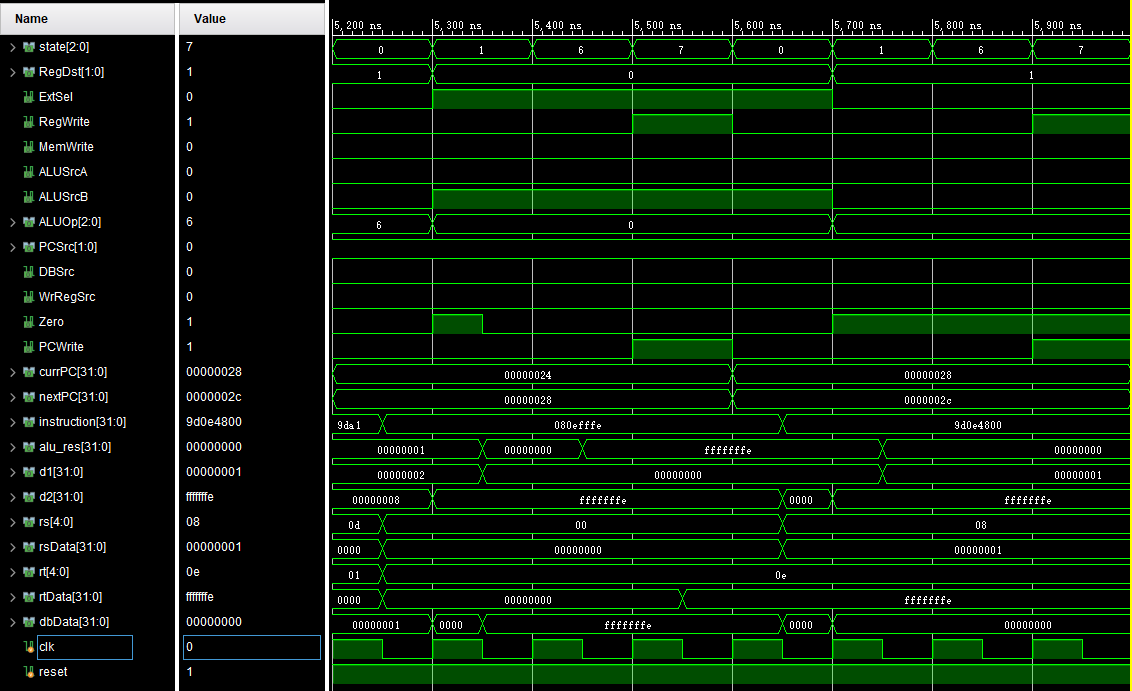
\includegraphics[width=0.9\linewidth]{fig/FullIns/Ins7.PNG}
\caption{波形图7}
\label{fig:wave_7}
\end{figure}
    \item \verb'0x24  addiu $14,$0,-2'\\
    在EXE(6)阶段算得Reg[0]+(-2)=\verb'0xFFFFFFFE',并在WB(7)存入Reg[14]
    \item \verb'0x28  slt $9,$8,$14'\\
    在EXE(6)阶段算得Reg[8]<Reg[14]=1<-2=0,并在WB(7)存入Reg[9]
\begin{figure}[H]
\centering
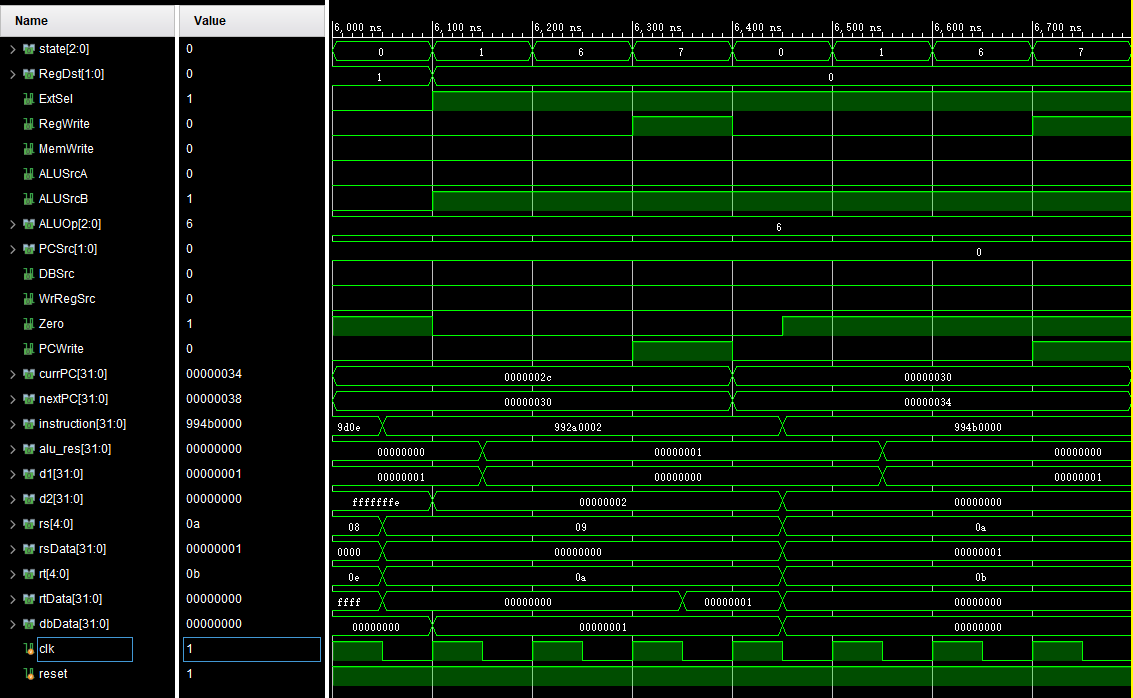
\includegraphics[width=0.9\linewidth]{fig/FullIns/Ins8.PNG}
\caption{波形图8}
\label{fig:wave_8}
\end{figure}
    \item \verb'0x2C  slti $10,$9,2'\\
    在EXE(6)阶段算得Reg[9]<2=0<2=1,并在WB(7)存入Reg[10]
    \item \verb'0x30  slti $11,$10,0'\\
    在EXE(6)阶段算得Reg[10]<=0=1<0=0,并在WB(7)存入Reg[11]
\begin{figure}[H]
\centering
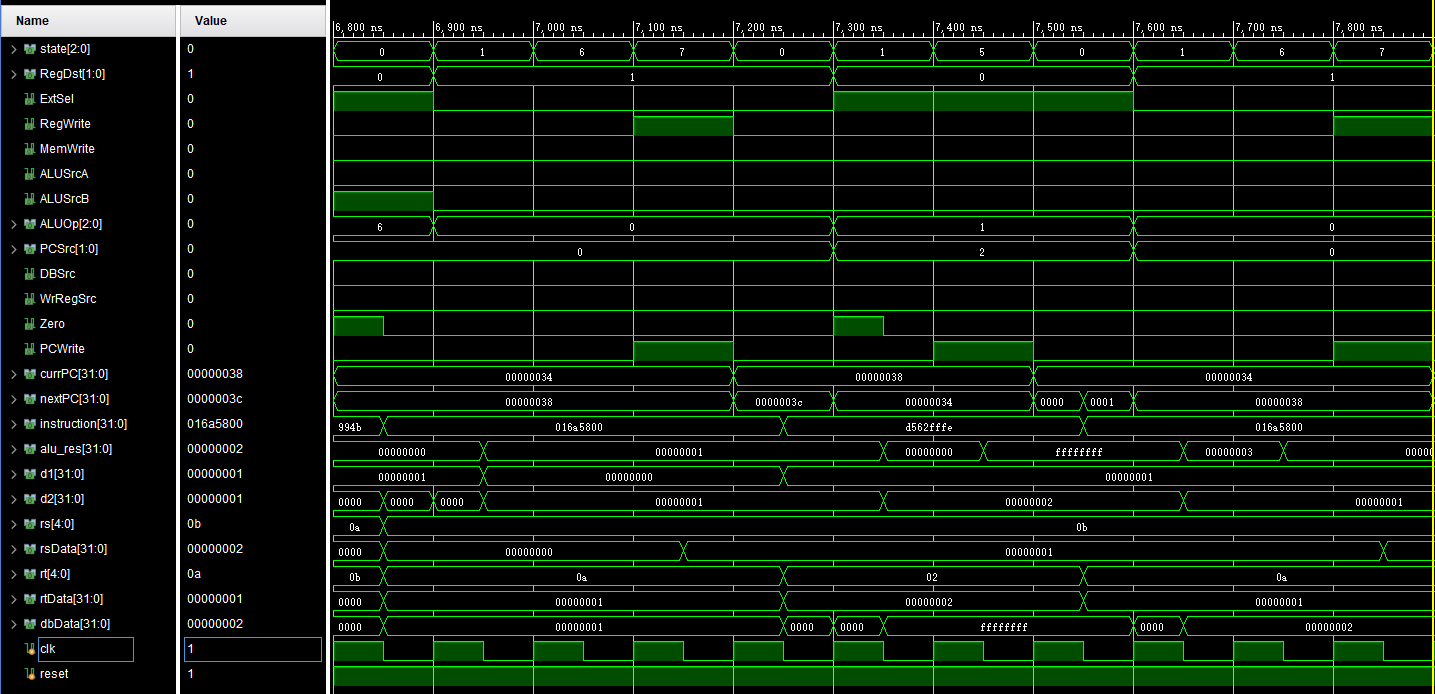
\includegraphics[width=0.9\linewidth]{fig/FullIns/Ins9.PNG}
\caption{波形图9}
\label{fig:wave_9}
\end{figure}
    \item \verb'0x34  add $11,$11,$10'\\
    在EXE(6)阶段算得Reg[11]+Reg[10]=0+1=1,并在WB(7)存入Reg[11]
    \item \verb'0x38  bne $11,$2,-2'\\
    在EXE(5)阶段算得Reg[11]-Reg[2]=1-2=-1=\verb'0xFFFFFFFF',不等于,跳转回\verb'0x34'
\begin{figure}[H]
\centering
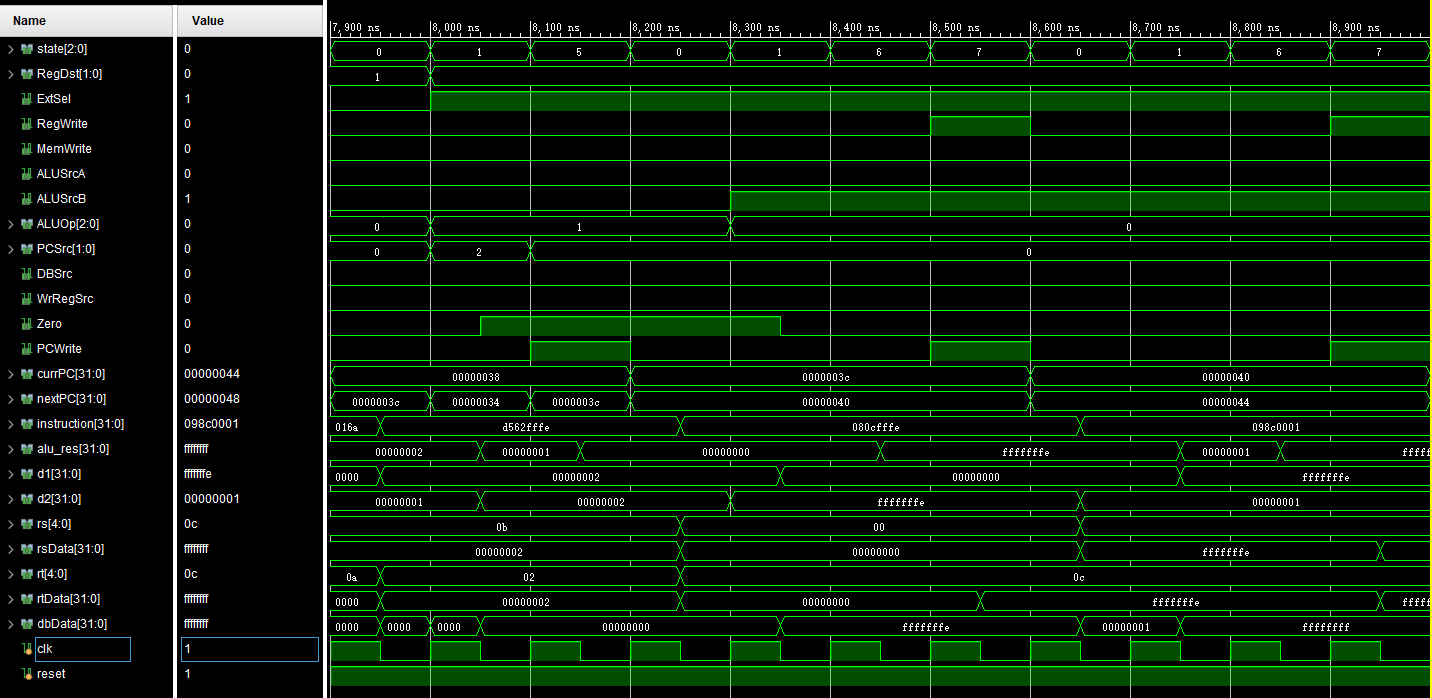
\includegraphics[width=0.9\linewidth]{fig/FullIns/Ins10.PNG}
\caption{波形图10}
\label{fig:wave_10}
\end{figure}
    \item \verb'0x34  add $11,$11,$10'\\
    在EXE(6)阶段算得Reg[11]+Reg[10]=1+1=2,并在WB(7)存入Reg[11]
    \item \verb'0x38  bne $11,$2,-2'\\
    在EXE(5)阶段算得Reg[11]-Reg[2]=2-2=0,相等,不跳转,执行下条指令
\begin{figure}[H]
\centering
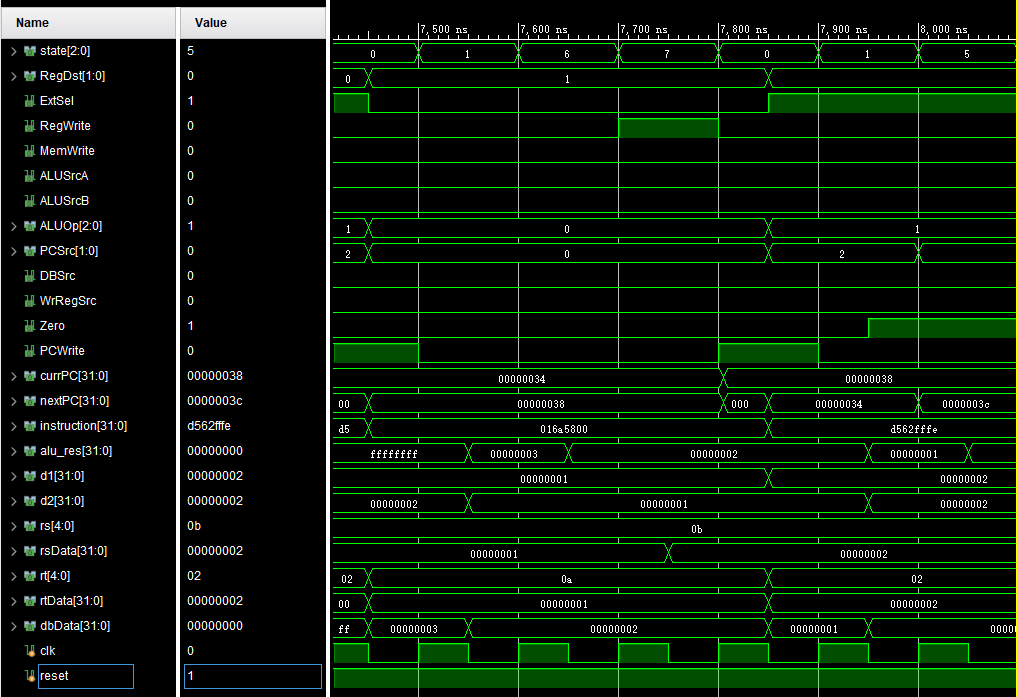
\includegraphics[width=0.9\linewidth]{fig/FullIns/Ins11.PNG}
\caption{波形图11}
\label{fig:wave_11}
\end{figure}
    \item \verb'0x3C  addiu $12,$0,-2'\\
    在EXE(6)阶段算得Reg[0]+(-2)=\verb'0xFFFFFFFE',并在WB(7)存入Reg[12]
    \item \verb'0x40  addiu $12,$12,1'\\
    在EXE(6)阶段算得Reg[12]+1=\verb'0xFFFFFFFF',并在WB(7)存入Reg[12]
\begin{figure}[H]
\centering
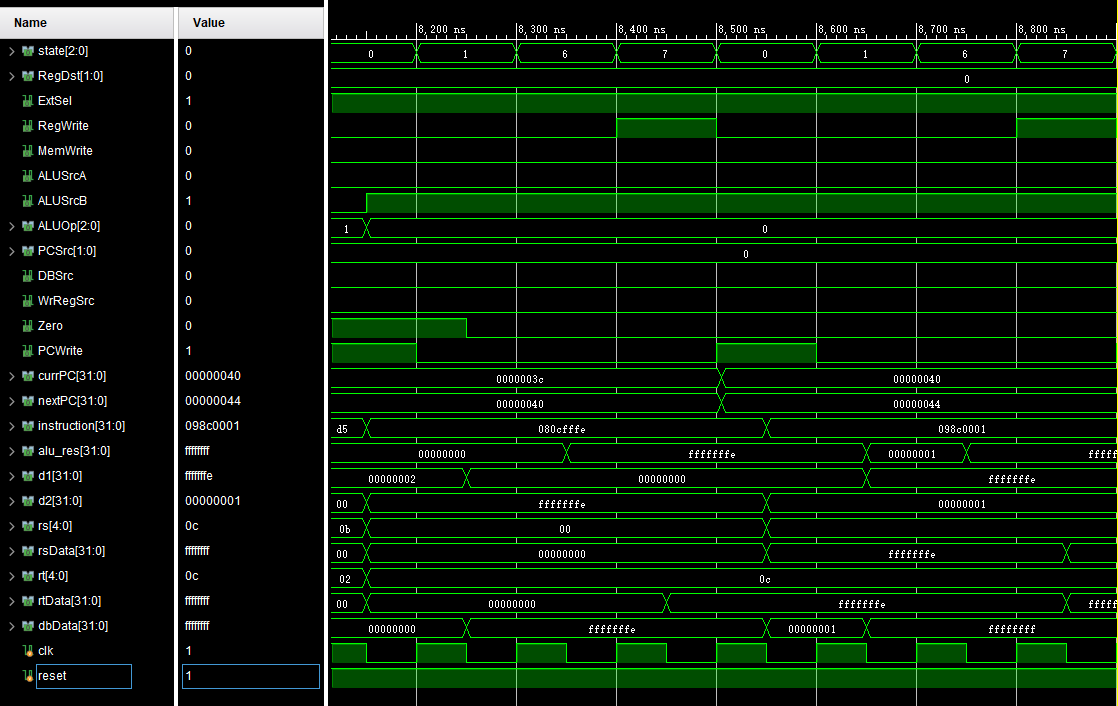
\includegraphics[width=0.9\linewidth]{fig/FullIns/Ins12.PNG}
\caption{波形图12}
\label{fig:wave_12}
\end{figure}
    \item \verb'0x44  bltz $12,-2'\\
    在EXE(5)阶段算得Reg[12]<0=-1<0=1,故跳转回\verb'0x40'
    \item \verb'0x40  addiu $12,$12,1'\\
    在EXE(6)阶段算得Reg[12]+1=0,并在WB(7)存入Reg[12]
\begin{figure}[H]
\centering
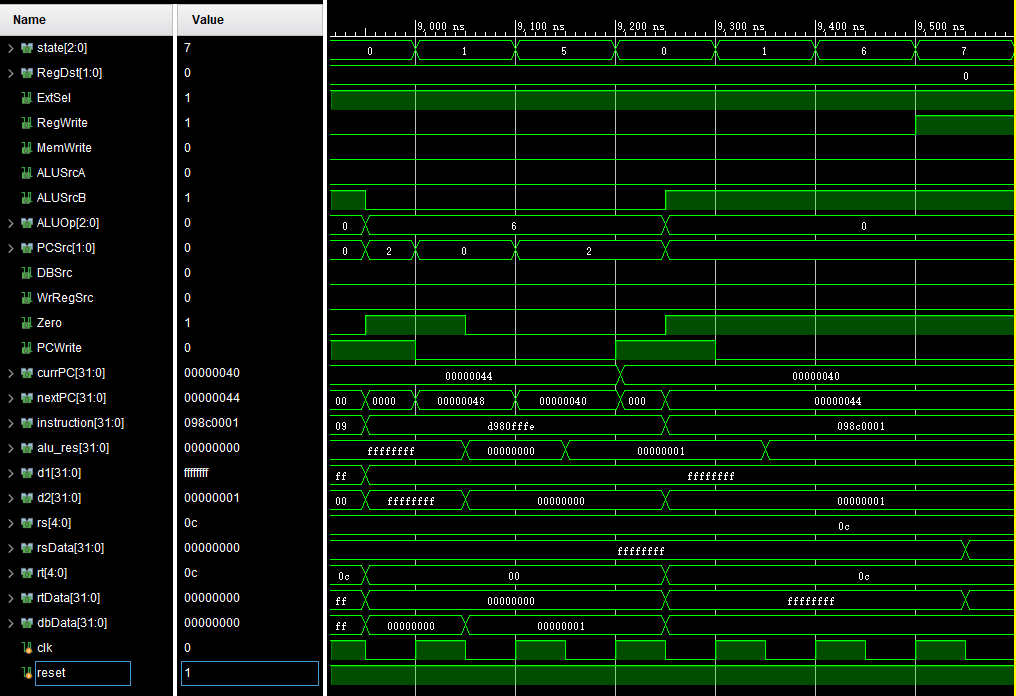
\includegraphics[width=0.9\linewidth]{fig/FullIns/Ins13.PNG}
\caption{波形图13}
\label{fig:wave_13}
\end{figure}
    \item \verb'0x44  bltz $12,-2'\\
    在EXE(5)阶段算得Reg[12]<0=0<0=0,故不跳转,继续执行下一指令
    \item \verb'0x48  andi $12,$2,2'\\
    在EXE(6)阶段算得Reg[2]\&2=2\&2=2,并在WB(7)存入Reg[12]
\begin{figure}[H]
\centering
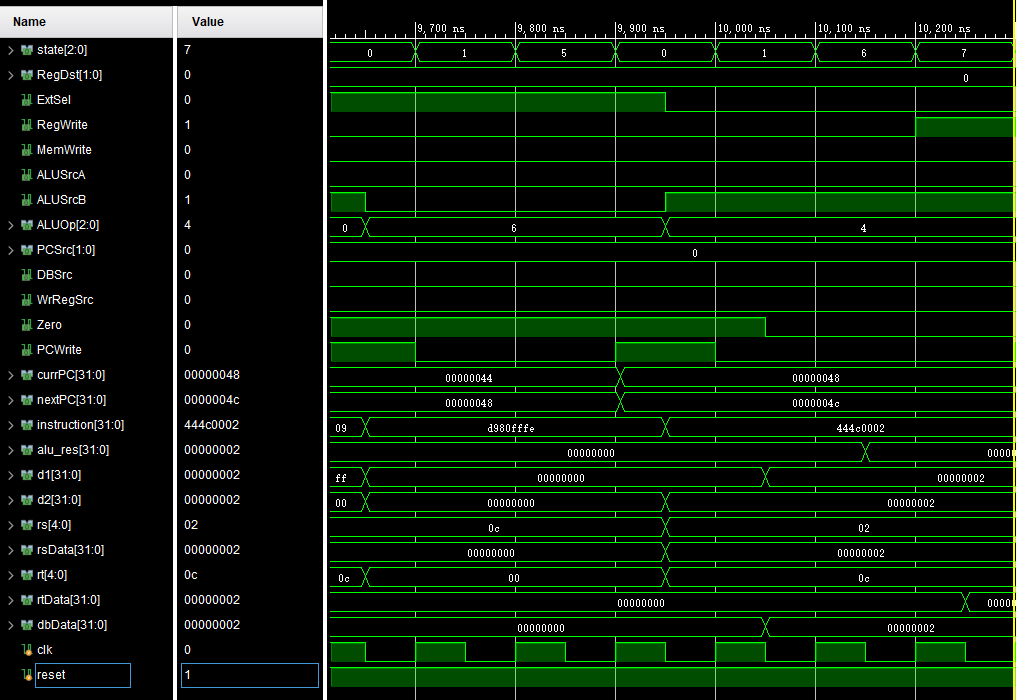
\includegraphics[width=0.9\linewidth]{fig/FullIns/Ins14.PNG}
\caption{波形图14}
\label{fig:wave_14}
\end{figure}
    \item \verb'0x50  j 0x000005C'\\
    在IF(0)后半阶段写入指令到IR,译码得出其为跳转指令,更新下一PC值为\verb'0x5C'
    \item \verb'halt'\\
    在ID(1)阶段求得指令为停机,不再更新PC
\begin{figure}[H]
\centering
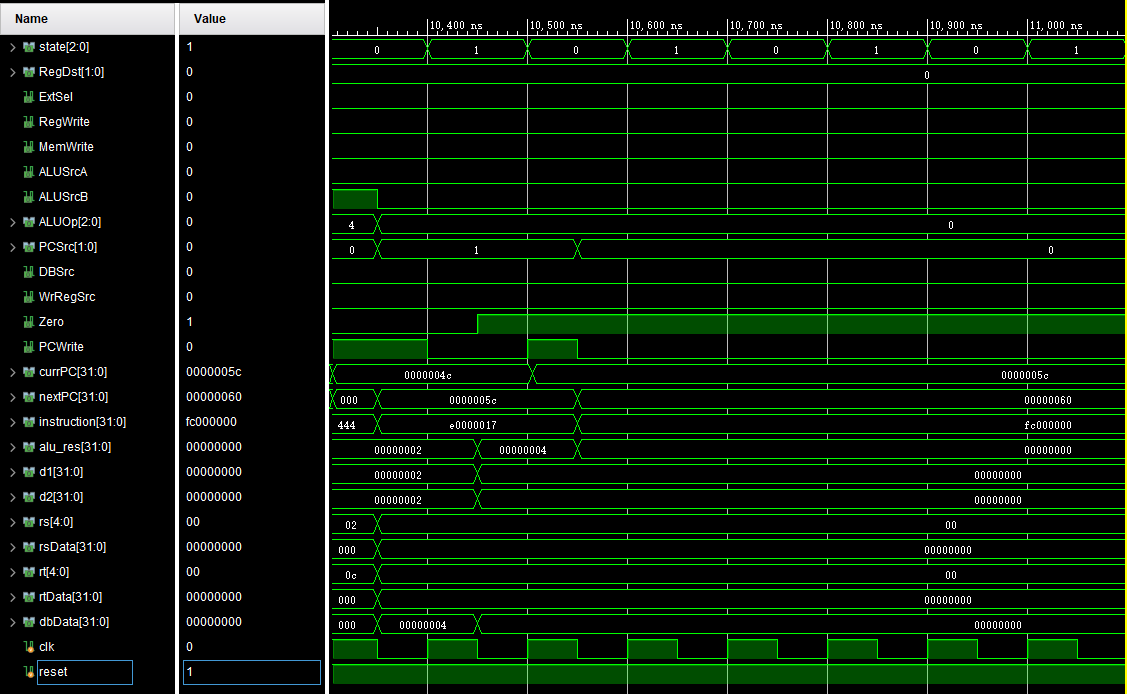
\includegraphics[width=0.9\linewidth]{fig/FullIns/Ins15.PNG}
\caption{波形图15}
\label{fig:wave_15}
\end{figure}
\end{enumerate}